\documentclass[10pt, a4paper, twoside, twocolumn]{book}
\usepackage{graphicx}

\title{ATHENS_Daily_Assignments}
\author{Mercedes Roman Ruiz}
\date{March 2026}

\renewcommand{\chaptername}{Assignment}
\usepackage[top = 2cm, bottom = 2cm, left = 2cm, right = 2cm, marginparwidth = 1.75cm]{geometry}
\usepackage[backend=biber, style=numeric, refsection=chapter]{biblatex}
\addbibresource{bibliografia.bib}
\usepackage{caption}
\captionsetup[figure]{font=small}
\usepackage{eurosym}
\usepackage{multirow}

\usepackage{fancyhdr}

\fancyhf{}
\pagestyle{fancy}
\fancyfoot[LO,RE]{Mercedes Román Ruiz}
\fancyfoot[LE,RO]{\thepage}
\fancyhead[LE,RO]{Flexibility in Power Systems (ATHENS KUL 39)}
\fancyhead[LO, RE]{Universidad Politécnica de Madrid}

\fancypagestyle{plain}{
    \fancyhf{} 
    \fancyfoot[LO]{Mercedes Román Ruiz}
    \fancyfoot[LE,RO]{\thepage} 
    \renewcommand{\headrulewidth}{0pt} 
}

\begin{document}

\chapter{Flexibility value chain stakeholders in Malta and discussion of implementable flexibility types}

Malta is a small and highly centralized island power system. In 2024, it supplied 3,106.1 GWh of electricity; 58.1\% came from power plants, 31.1\% from net imports through the Sicily interconnector, and 10.8\% from renewable sources. Since 97.2\% of renewable electricity came from solar PV, Malta’s flexibility challenge is mainly linked to solar variability, imports, and the operational constraints of a small island system \cite{nso_electricity_2025}.

\begin{figure}[h]
    \centering
    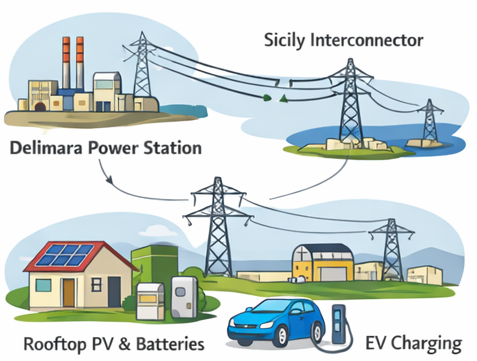
\includegraphics[width=\columnwidth]{malta_power_system_overview.png}
    \caption{Simplified overview of Malta’s power system and flexibility-relevant assets.}
\end{figure}

\section{Flexibility value chain stakeholders in Malta}

\paragraph{Distribution System Operator (DSO): Enemalta plc.} Enemalta is the key actor in Malta’s electricity system, since it operates the distribution grid and remains the sole electricity supplier to final consumers \cite{ewa_necp_2025,enemalta_services_2026}.

\paragraph{Transmission System Operator (TSO): no separate TSO exists in Malta.} Malta has no electricity transmission system and therefore no separate TSO; instead, Enemalta performs some TSO-like functions, including central dispatch and operation of the Sicily interconnector \cite{ewa_necp_2025}.

\paragraph{Market operator: no separate domestic wholesale market operator is currently present.} Malta does not have a liquid domestic wholesale electricity market, so it also lacks a distinct national market operator comparable to EPEX SPOT or Nord Pool \cite{ewa_necp_2025}.

\paragraph{Aggregator: an emerging rather than mature stakeholder.} The aggregator role in Malta is still weak. The NECP states that there are no successful local demand-response business models yet, although second-generation smart meters may support aggregation in the future \cite{ewa_necp_2025}.

\paragraph{Flexibility providers: households, EV users, commercial and industrial users, and storage owners.} The most realistic providers are rooftop PV prosumers, users with behind-the-meter batteries, EV charging users, and larger commercial consumers. By the end of 2023, Malta had 775 behind-the-meter battery systems with 6.03 MWh of capacity \cite{ewa_necp_2025}.

\paragraph{Consumers and prosumers.} Consumers in Malta are still mostly exposed to regulated tariffs rather than dynamic market prices, while prosumers are mainly PV owners, increasingly combined with storage \cite{ewa_necp_2025,rews_tariffs_2025}.

\paragraph{Bulk generation companies.} The main bulk generation actors are ElectroGas Malta, D3 Power Generation, and Enemalta’s backup and emergency generation assets \cite{ewa_necp_2025}.

\begin{figure}[h]
    \centering
    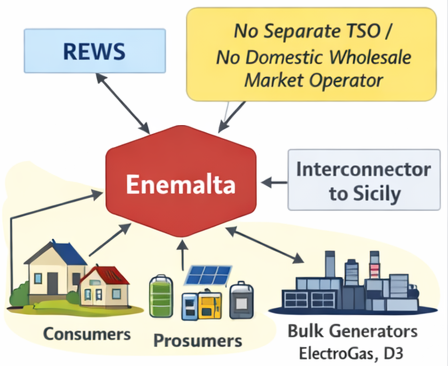
\includegraphics[width=\columnwidth]{malta_stakeholder_diagram.png}
    \caption{Main stakeholders in Malta’s flexibility value chain.}
\end{figure}

\section{Discussion of flexibility types implementable in Malta}

According to the course framework, Type I refers to explicit availability with direct management, Type II to explicit availability with indirect management, Type III to implicit availability with indirect management, and Type IV to implicit availability with direct management.

\begin{figure}[h]
    \centering
    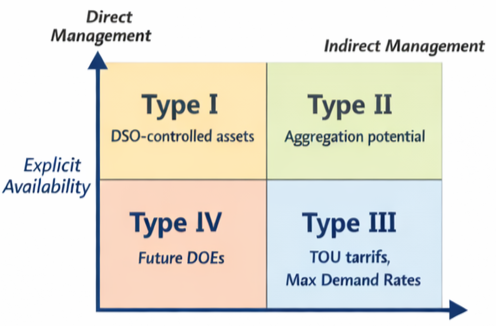
\includegraphics[width=\columnwidth]{malta_flexibility_types_matrix.png}
    \caption{Interpretation of flexibility types I--IV for the Maltese case.}
\end{figure}

\paragraph{Type I -- implementable, but limited.} Type I is feasible mainly through centrally managed assets and technical requirements imposed on connected devices, such as Volt-Var settings for non-synchronous inverters and utility-scale battery storage \cite{enemalta_techspec_2025,ewa_necp_2025}.

\paragraph{Type II -- technically possible, but commercially weak.} Malta has some technical ingredients for Type II, including storage, EVs and future V2G. However, the current market structure is not yet conducive to mature demand-response and aggregation services \cite{ewa_necp_2025}.

\paragraph{Type III -- the most realistic near-term option.} Type III is the most implementable in the short term because Malta already combines very high smart-meter deployment with tariff-based incentives, especially for larger users and EV charging \cite{ewa_necp_2025,rews_tariffs_2025}.

\paragraph{Type IV -- promising, but not yet mature.} Type IV could become relevant as Malta advances smart-grid digitalisation, second-generation smart meters and near-real-time data capabilities. However, there is still no evidence of a fully established nationwide dynamic operating envelope scheme \cite{ewa_necp_2025}.

\section{Conclusion}

Malta’s flexibility value chain is more centralized than in larger EU electricity systems. Enemalta dominates the chain, there is no separate TSO, and the aggregator role remains underdeveloped. As a result, Type III and selected Type I applications appear to be the most realistic options today, while broader Type II and Type IV approaches still depend on further digitalisation, stronger business models and market reform \cite{ewa_necp_2025}.

\printbibliography[heading=subbibliography, title={References}]

\chapter{Smart metering in Malta}

Malta provides an interesting case for smart metering because it is a small island power system with a relatively advanced level of digitalisation in electricity metering. However, when analysing smart metering penetration, it is important to distinguish between meters that are simply installed and meters that are fully connected and reachable remotely through the utility's Automatic Metering Management system. According to the 2025 report of the Regulator for Energy and Water Services (REWS), by the end of 2024 Malta had 358,002 smart meters reachable remotely out of 388,161 active meters, corresponding to 92.23\% of all active meters. For households, the figure was 308,985 remotely reachable smart meters out of 331,876 active household meters, which represents 93.10\%. This confirms that Malta has a high level of smart metering penetration, although a small share of the installed fleet is still not fully integrated into remote communications and automatic meter management \cite{rews_nationalreport_2025}.

\begin{figure}[h]
    \centering
    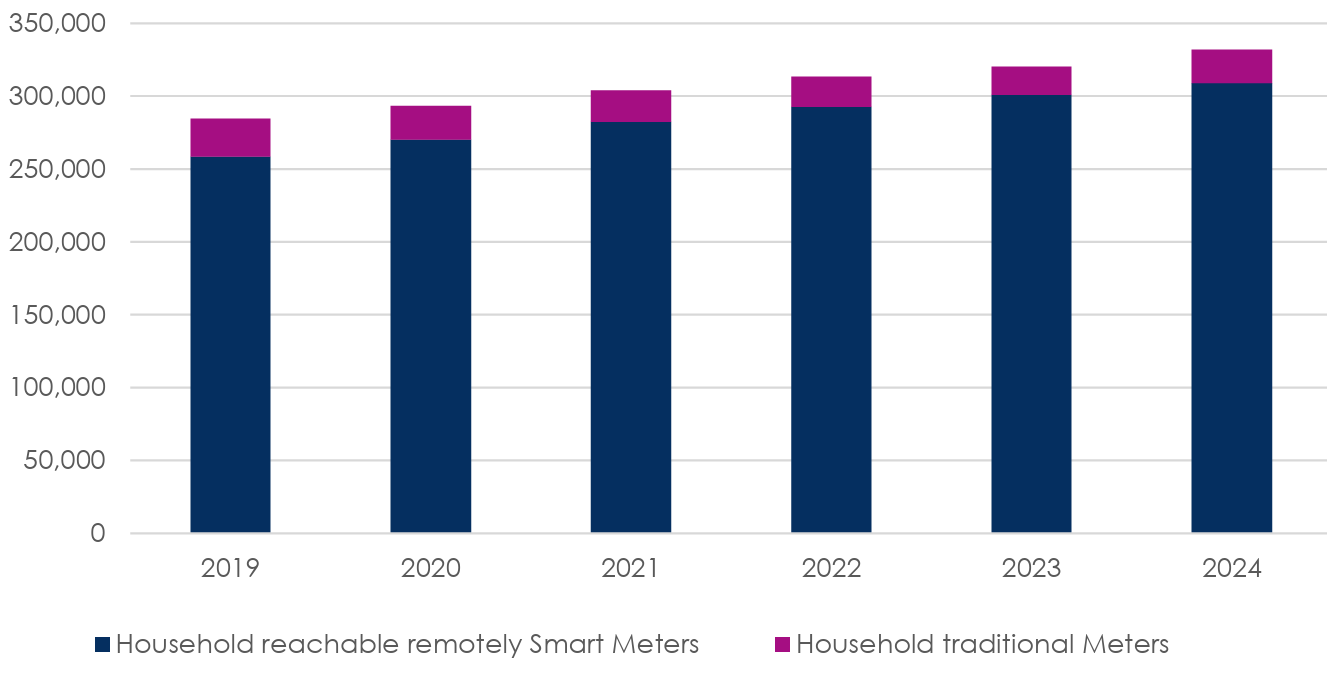
\includegraphics[width=\columnwidth]{malta_smart_meter_rollout.png}
    \caption{Household smart meter development between 2019 and 2024 \cite{rews_nationalreport_2025}.}
\end{figure}

The main meter types used in Malta are differentiated according to the type of electrical connection. ARMS and Enemalta identify three main smart meter categories in the first-generation rollout: GISM for single-phase customers, GIST for three-phase customers, and GISS for heavy consumers. This already shows that the Maltese system is not based on a single universal residential meter, but on different devices depending on user profile and connection requirements. In addition, Enemalta has started introducing second-generation smart meters, and in 2024 it announced the installation of GESIS, a CT-operated smart meter for bulk commercial and industrial supplies. This suggests that Malta is gradually moving from a first-generation remote metering system toward a more advanced AMI environment with improved flexibility and monitoring capabilities \cite{arms_faqs_2026,enemalta_smartmeters_faq_2018,enemalta_gesis_2024}.

\begin{figure}[h]
    \centering
    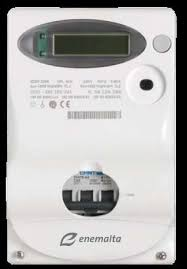
\includegraphics[width=0.5\columnwidth]{enamalta_smart_meter.png}
    \caption{Example of an Enemalta smart meter \cite{arms_smartmeter_manual_2018}.}
\end{figure}

Regarding the data measured, Maltese sources show that the system is primarily focused on billing accuracy, demand monitoring, prosumer settlement and remote utility operations. The REWS national report states that Maltese smart meters provide remote spot readings for import and export registers, maximum demand and load profiles, as well as time-of-use consumption readings. The same report also confirms remote activation and deactivation and remote power-limit curtailment as available functionalities. The customer smart meter manual complements this by showing that the display can provide instantaneous power, total accumulated consumption, current-period consumption, today’s consumption, tariff-related readings, maximum demanded power and, where relevant, exported energy from photovoltaic generation. Enemalta also explicitly states that the meter records both imported and exported energy for customers who generate electricity. For newer meter families used in commercial and industrial contexts, publicly available conformity documents refer to active and reactive energy measurement. By contrast, I did not find strong public evidence that voltage, current or frequency are systematically exposed as standard customer-facing variables across the whole national fleet, so I would avoid overstating that point \cite{rews_nationalreport_2025,arms_smartmeter_manual_2018,enemalta_smartmeters_faq_2018,gridspertise_gemis_red_2021,gridspertise_gesis_red_2021}.

A second relevant aspect is the difference between local measurement update, remote data collection and final billing frequency. In Malta, these three levels should not be confused. According to the user manual, instantaneous power on the meter display corresponds to the average power demanded during the previous two minutes and is automatically updated every two minutes. Enemalta also states that smart meters can be read very frequently, even up to every 15 minutes, which indicates that quarter-hour data granularity is available at system level. However, this does not mean that customers are billed every 15 minutes. REWS explains that households whose smart meters are connected to the Automatic Metering Management system receive bills based on actual readings on a bimonthly basis, while non-household consumers receive actual bills with frequencies ranging from one to six months. ARMS also notes that after installation, the time required for a meter to become permanently connected to the central system may vary between four weeks and three months, depending on the area. Therefore, Malta combines relatively fine measurement granularity with slower commercial settlement cycles \cite{arms_smartmeter_manual_2018,enemalta_smartmeters_faq_2018,rews_nationalreport_2025,arms_faqs_2026}.

The communication layer is the point where the public information becomes less transparent. Official Maltese consumer-facing sources clearly state that the smart meter transmits data through a network to a central system and can receive commands remotely, but they do not fully disclose the exact nationwide communication architecture of the original large-scale rollout. What is explicitly documented is the presence of a local optical interface on the meter for authorised technical personnel. For the newer second-generation Gridspertise family now being introduced in Malta, the documentation is more informative. The vendor platform supports multiple communication options such as PLC, RF mesh, LTE and NB-IoT, and the conformity documents for GEMIS and GESIS refer to radio-based communication, including short-range operation in the 169.400--169.475~MHz band. This suggests that Malta is evolving toward a more flexible multi-technology AMI architecture, even if the exact mix of communication media in the full deployed fleet is not publicly described in detail. From an engineering perspective, this is an important limitation because communication performance strongly affects the potential use of smart metering for flexibility services, demand response and low-voltage grid observability \cite{enemalta_smartmeters_faq_2018,arms_smartmeter_manual_2018,gridspertise_residentialmeters_2026,gridspertise_gemis_red_2021,gridspertise_gesis_red_2021}.

Overall, Malta can be considered a relatively mature smart metering case within Europe, especially in terms of remote reachability, prosumer measurement and operational utility functions. Its strengths are the high share of remotely reachable meters, the ability to distinguish import and export flows, the availability of maximum demand and load-profile data, and the existence of remote service functions such as activation, disconnection and power-limit control. These features are already relevant for a future flexibility-oriented power system. At the same time, the public documentation shows that a distinction must still be made between installed smart meters and remotely reachable meters, and that the exact communication structure of the whole legacy fleet remains insufficiently transparent in public sources. For this reason, Malta appears technically well positioned for further smart-grid development, but still with room for improvement in communication transparency and data accessibility \cite{rews_nationalreport_2025,enemalta_services_2026,ewa_necp_2025}.

\printbibliography[heading=subbibliography, title={References}]

\chapter{Flexibility needs in Malta under large-scale DER adoption}

Malta is a small island electricity system with no domestic transmission system and no separate TSO; in practice, the DSO has a central operational role and is also responsible for balancing \cite{ewa_necp_2025}. In 2024, Malta supplied 3,106.1~GWh of electricity and reached a peak demand of 593~MW. Renewable sources accounted for 10.8\% of electricity supply, and 97.2\% of renewable electricity came from PV. Installed renewable capacity reached 255.14~MW by the end of 2024, while grid-connected PV amounted to 252,255.4~kWp across 34,955 installations \cite{nso_electricity_2025,rews_nationalreport_2025,nso_pv_2025}. As a result, Malta’s flexibility challenge is strongly linked to solar variability, local network stress and the operational constraints of a relatively small and centralised power system.

\begin{figure}[h]
    \centering
    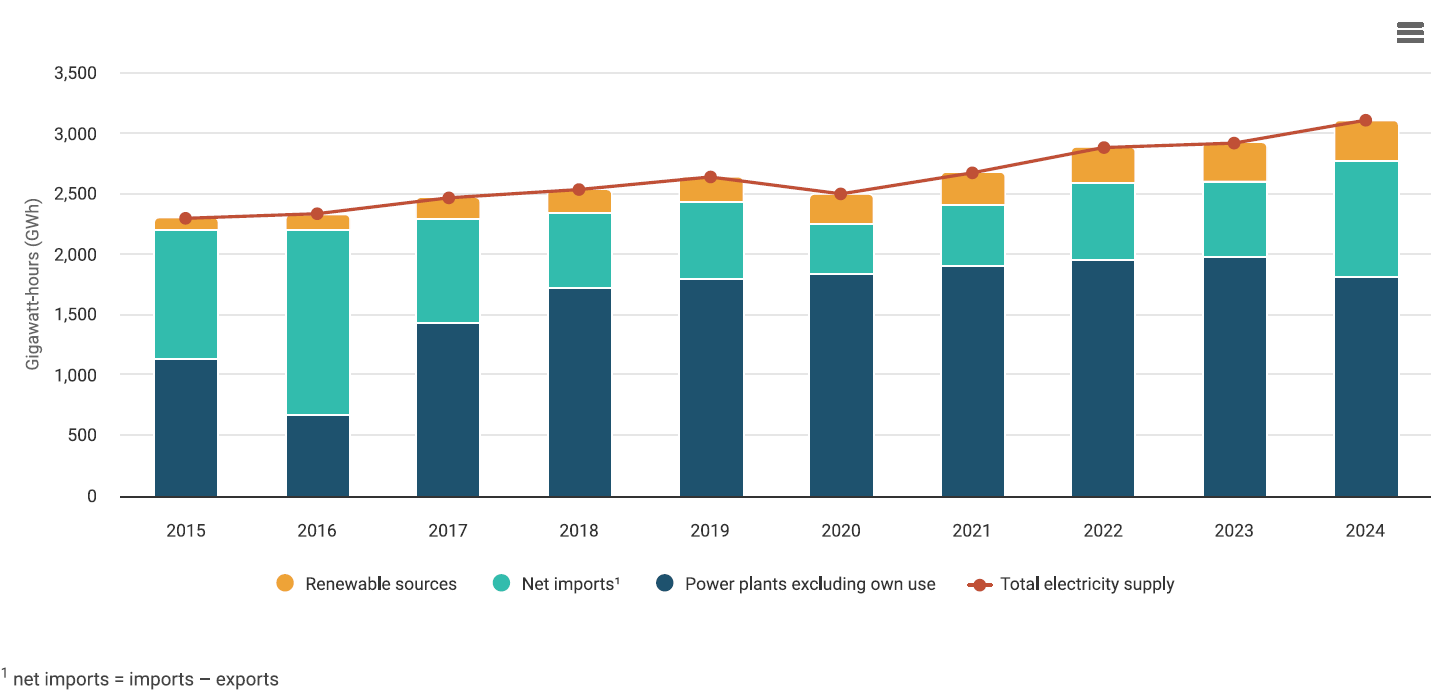
\includegraphics[width=\columnwidth]{malta_electricity_supply_2015_2024.png}
    \caption{Electricity supply in Malta by source, 2015--2024 \cite{nso_electricity_2025}.}
\end{figure}

\section{System outlook and high-DER scenario}

The updated Maltese NECP projects solar PV capacity to reach 350~MWp by 2030 and transport electrification to the equivalent of almost 65,000 electric and plug-in hybrid passenger cars, supported by around 6,500 charging points \cite{ewa_necp_2025}. This means that Malta’s 2030 electricity system is expected to have substantially higher DER penetration, especially in rooftop PV and flexible electrical demand associated with mobility.

A relevant enabling factor is metering and digitalisation. Malta already has a very high smart-meter rollout, and the NECP reports that 99.6\% of consumers were equipped with first-generation smart meters, while second-generation rollout stood at around 17.8\% of installed smart meters \cite{ewa_necp_2025}. However, near-real-time data access and full demand-response functionality still require further upgrades in metering and IT systems. Therefore, Malta has a solid observability base, but not yet a fully mature flexibility activation framework.

This 2030 scenario is important because Malta’s electricity system is not only decarbonising but also becoming more dynamic. In larger continental systems, transmission, balancing and distribution constraints may be more separated. In Malta, by contrast, voltage problems, reverse power flows, peak management and short-term balancing can all emerge together. This makes flexibility particularly valuable as a system-wide tool rather than as a narrow congestion-management instrument.

\section{Main challenges under large-scale DER adoption}

The clearest flexibility driver in Malta is short-term PV variability. The NECP reports that with 236~MWp of installed PV at the end of 2023, Malta experienced transients of about 95~MW within 30 minutes, while PV penetration during low-demand Sunday afternoons in April 2023 reached around 57\% of demand \cite{ewa_necp_2025}. If this behaviour is scaled to the 2030 target of 350~MWp, Malta should be prepared to manage PV ramps of roughly 140~MW in 30 minutes. For a system whose 2024 peak demand was 593~MW, this is already a very material operational requirement.

A second challenge is the coexistence of midday PV surplus and evening electrified demand. On sunny low-demand periods, Malta will increasingly need to absorb local surplus generation to avoid curtailment and stress on low-voltage feeders. By contrast, in evening hours, EV charging and other electrified demand may intensify the peak unless charging is shifted away from those periods. In other words, the flexibility need is both downward and upward, depending on the time of day.

A third challenge is institutional. The NECP explicitly states that Malta does not yet have a liquid wholesale electricity market and that the present market structure is not conducive to mature demand-response participation \cite{ewa_necp_2025}. Therefore, Malta’s flexibility problem is not only technical. The country may have flexible assets, but it still needs the market, digital and regulatory conditions required to mobilise them efficiently.

\begin{figure}[h]
    \centering
    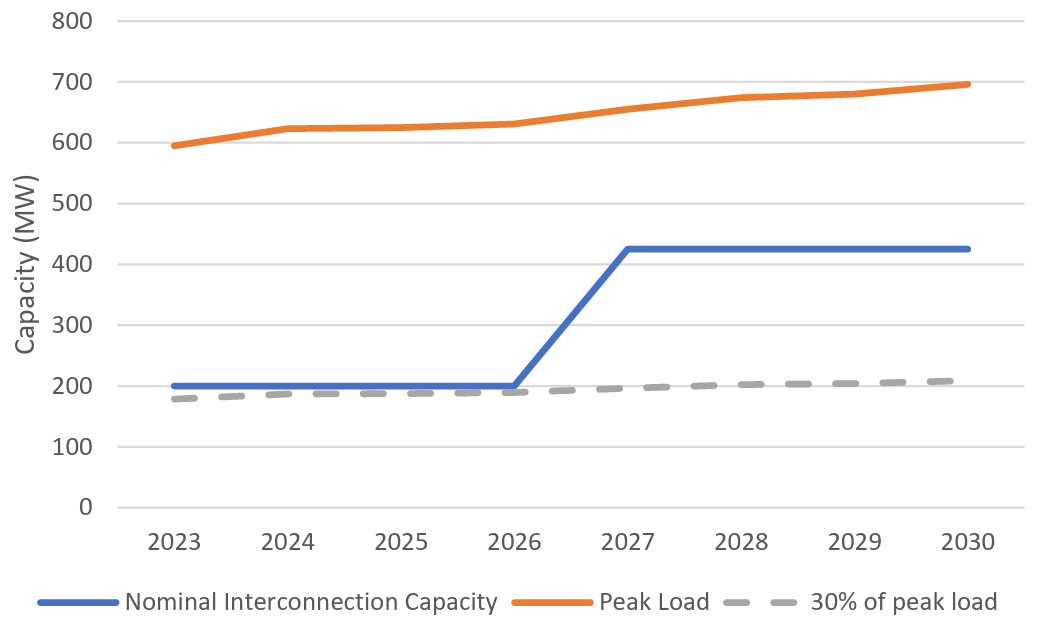
\includegraphics[width=\columnwidth]{malta_interconnection_peakload_2023_2030.png}
    \caption{Projected interconnection capacity, peak load and 30\% peak-load threshold in Malta, 2023--2030 \cite{ewa_necp_2025}.}
\end{figure}

\section{Indicative flexibility needs and potential}

The values presented here are indicative planning ranges rather than official Maltese FNA results. For 2030, Malta is likely to need around 90--140~MW of downward flexibility during sunny, low-demand periods, mainly to absorb PV surplus and reduce curtailment risk. Upward flexibility, understood as load reduction, storage discharge or equivalent fast balancing response, is likely to be in the range of 60--100~MW during evening peaks and sudden PV drops \cite{ewa_necp_2025,nso_electricity_2025}. In energy terms, this corresponds roughly to 100--250~MWh of intraday flexibility on critical days.

Since Malta has no domestic transmission system, most of this flexibility need is effectively distribution-level or DSO-facing rather than classical TSO-level congestion management \cite{ewa_necp_2025,rews_nationalreport_2025}. This is a key point: the flexibility challenge in Malta is not primarily about a large interconnected wholesale system, but about making a small island system more adaptable under rising DER penetration.

Malta does have promising flexibility resources, but they need to be activated. The NECP identifies two utility-scale battery projects, one of 8~MW / 20~MWh and another of 32~MW / 64~MWh, for a combined total of 40~MW / 84~MWh \cite{ewa_necp_2025}. This is an important step, but insufficient on its own for a 120--140~MW PV-ramp event. EV smart charging is also likely to become a major flexible resource by 2030; based on the national target of almost 65,000 electric and plug-in hybrid passenger cars, a conservative engineering estimate is that controllable charging could provide around 55--65~MW of shiftable demand. Malta also had 775 behind-the-meter battery systems with 6.03~MWh of capacity by the end of 2023, showing that distributed storage is emerging, although it remains supplementary at system scale \cite{ewa_necp_2025}. Additional support may come from commercial demand response, HVAC, water heating and smart inverter control.

\section{Conclusion}

Malta does not simply need more DER capacity; it needs accessible, observable and controllable flexibility to integrate that capacity securely. Based on current data and 2030 targets, Malta is likely to require approximately 90--140~MW of downward flexibility, 60--100~MW of upward flexibility and fast ramping capability close to 140~MW within 30 minutes. The challenge is mainly distribution-level and closely tied to PV variability, electrified demand growth and the limitations of Malta’s current market design.

The encouraging point is that Malta already has several relevant building blocks: strong PV deployment, very high smart-meter penetration, planned battery storage and rising EV electrification. However, unless second-generation metering, near-real-time data access, smart charging, aggregation and explicit demand-response models advance further, Malta will remain too reliant on the interconnector, conventional generation and curtailment under stressed conditions \cite{ewa_necp_2025,nso_electricity_2025,rews_nationalreport_2025,nso_pv_2025}.

\printbibliography[heading=subbibliography, title={References}]

\chapter{Compare grid investment needs vs flexibility planning cost in Malta}

Malta is a small island electricity system with limited indigenous energy resources and a strong dependence on imports, local thermal generation and solar PV \cite{ewa_necp_2025,nso_electricity_2025}. In 2024, Malta supplied 3,106.1~GWh of electricity, while peak demand on the distribution network reached 593.2~MW \cite{nso_electricity_2025,rews_nationalreport_2025}. Looking ahead, the REWS national report reproduces the DSO forecast of annual electricity demand rising to 3,666,691~MWh by 2030 \cite{rews_nationalreport_2025}. At the same time, Malta's updated NECP targets around 350~MW of land-based PV by 2030 and continued electrification of transport \cite{ewa_necp_2025}. Therefore, Malta must decide how much of this transition should be accommodated through traditional network reinforcement and how much through flexibility-based solutions.

\begin{figure}[h]
    \centering
    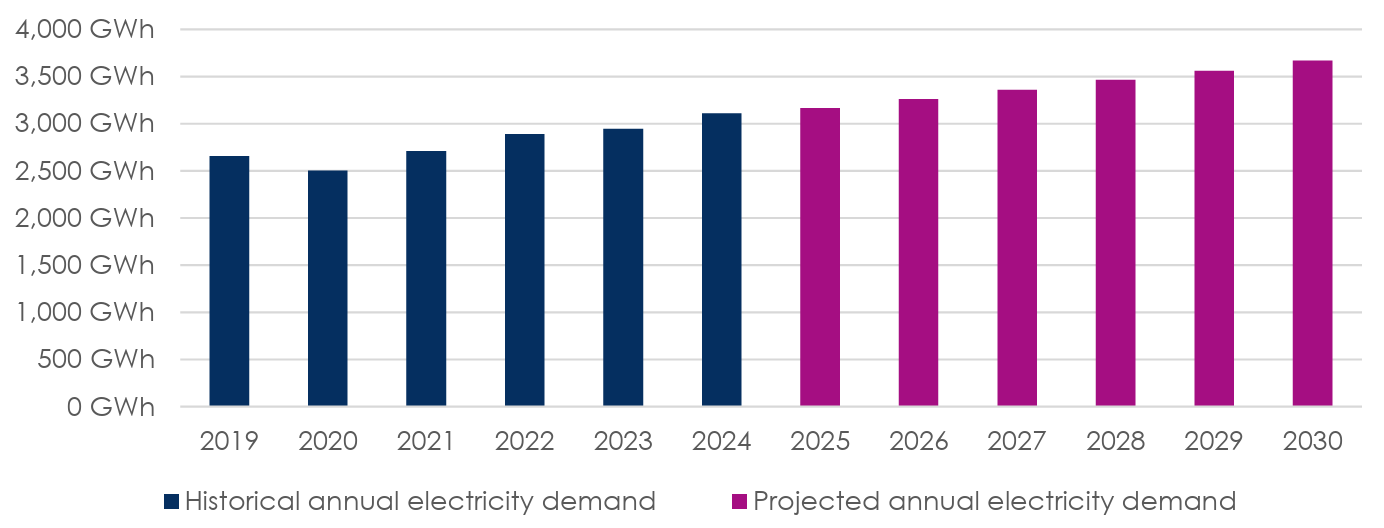
\includegraphics[width=\columnwidth]{rews_figure6_demand_forecast.png}
    \caption{Historical and projected annual electricity demand in Malta \cite{rews_nationalreport_2025}.}
\end{figure}

\section{Grid investment needs in Malta}

The most clearly documented large-scale grid investment in Malta is the second Malta--Sicily electricity interconnector (IC2). According to official Maltese sources, this project is a strategic backbone reinforcement intended to strengthen security of supply, support demand growth and facilitate further renewable integration \cite{gov_ic2_2025,ewa_necp_2025}. In Malta's case, this type of investment is especially important because the system is small, centralised and vulnerable to adequacy and resilience issues that cannot be solved only through flexible demand or behind-the-meter assets.

\begin{table}[h]
    \centering
    \caption{Technical parameters for the second electricity interconnector. Source: ICM \cite{ewa_necp_2025}}
    \resizebox{\columnwidth}{!}{
    \begin{tabular}{| c | c | c | c |}
        \hline
        \multicolumn{4}{|c|}{Main Technical Parameters}\\
        \hline
        Type & Approx. route length & Capacity & Nominal Voltage \\
        50Hz - HVAC cable & 122 km & 225 MW & 220 kV \\
        \hline
    \end{tabular}
    }
\end{table}

The scale of this investment is also consistent with Malta's recent security-of-supply decisions. The REWS national report notes that a temporary 60~MW diesel backup plant was licensed in 2024 to support peak demand and system constraints until the new cable becomes operational \cite{rews_nationalreport_2025}. This reinforces the idea that conventional infrastructure is still necessary in Malta. Flexibility may optimise the system, but it cannot fully replace the role of backbone network reinforcement in a small island grid.

\section{Flexibility planning costs}

Publicly documented flexibility-enabling investments are much smaller in size. The clearest example is the public tender for two utility-scale Battery Energy Storage Systems (BESS) in Marsa and Delimara, with an estimated contract value of \euro47~million excluding VAT \cite{eu_bess_tender_2024}. The REWS national report also explains that Malta first attempted to procure flexibility services through battery storage, but that this initial commercial process revealed market failure because financial offers were above the willingness-to-pay \cite{rews_nationalreport_2025}. The country then moved towards publicly backed BESS procurement.

The updated NECP also identifies smaller flexibility-related measures. While the NECP reports more than \euro100~million of additional planned investment up to 2030 mainly for PV expansion and active mobility, one directly relevant measure is the Green Mobility Scheme, with an estimated cost of \euro7.5~million, supporting cleaner fleets and EV-related infrastructure for business operations \cite{ewa_necp_2025}. Malta also already applies dedicated off-peak EV charging tariffs, which are not capital-intensive but are important because they create low-cost operational flexibility by shifting part of EV charging away from stressed periods \cite{rews_tariffs_2025}.

\section{Economic comparison}

The cost contrast is therefore very clear. The \euro47~million BESS package corresponds to only a small share of the roughly \euro300~million second interconnector \cite{gov_ic2_2025,eu_bess_tender_2024}. Even when smaller flexibility-enabling measures are added, flexibility planning remains substantially cheaper than strategic grid reinforcement. From a short-run financial perspective, flexibility is therefore the lower-cost option.

However, the two options do not solve the same problem. Grid reinforcement is more expensive, but it delivers firm capacity, stronger security of supply and long-term system resilience. Flexibility solutions are cheaper and more modular, but they are better suited to operational optimisation: peak shaving, midday PV absorption, EV charging management, local congestion relief and the deferral of some lower-voltage reinforcements. In Malta, where system adequacy and resilience remain critical, the appropriate conclusion is not to replace grid investment with flexibility, but to use flexibility as the first optimisation layer around a reinforced backbone network.

\section{Conclusion}

At national scale, Malta still needs major grid investment. The second interconnector is the clearest proof that strategic reinforcement remains essential for security of supply, redundancy and large-scale renewable integration. Nevertheless, flexibility planning is much cheaper in public cost terms and is better suited to solving the operational problems created by growing PV, EV charging and other distributed loads.

Therefore, Malta should not rely only on one of the two options. The most suitable strategy is a hybrid one: traditional grid reinforcement for backbone adequacy and resilience, combined with a stronger flexibility layer for local congestion management, peak shaving and renewable integration. In economic terms, flexibility should be prioritised before many smaller local upgrades, but it should complement, not replace, major network reinforcement projects \cite{gov_ic2_2025,eu_bess_tender_2024,ewa_necp_2025,rews_nationalreport_2025}.

\printbibliography[heading=subbibliography, title={References}]

\end{document}